% !TEX program = xelatex
% !TEX encoding = UTF-8 Unicode
\documentclass[aspectratio=169, 10pt]{beamer}

% ── Theme ────────────────────────────────────────────────────────────────────
\usetheme{Madrid}
\usecolortheme{default}
\usefonttheme{professionalfonts}

% ── Packages ─────────────────────────────────────────────────────────────────
\usepackage{booktabs}
\usepackage{array}
\usepackage{tikz}
\usetikzlibrary{arrows.meta, shapes.geometric, positioning, fit, backgrounds, calc, decorations.pathreplacing}
\usepackage{xcolor}
\usepackage{fontawesome5}
\usepackage{listings}
\usepackage{tabularx}
\usepackage{multirow}
\usepackage{xeCJK}
\setCJKmainfont{PingFang SC}
\setCJKsansfont{PingFang SC}
\setCJKmonofont{PingFang SC}

% ── Colors ───────────────────────────────────────────────────────────────────
\definecolor{darkblue}{RGB}{0,51,102}
\definecolor{lightblue}{RGB}{173,214,235}
\definecolor{llm1color}{RGB}{70,130,180}
\definecolor{llm2color}{RGB}{60,150,100}
\definecolor{judgecolor}{RGB}{180,80,60}
\definecolor{codegreen}{RGB}{40,120,60}
\definecolor{codegray}{RGB}{100,100,100}
\definecolor{alertred}{RGB}{200,50,50}
\definecolor{stepbg}{RGB}{240,245,255}

\setbeamercolor{frametitle}{bg=darkblue, fg=white}
\setbeamercolor{title}{bg=darkblue, fg=white}
\setbeamercolor{subtitle}{fg=white!85!darkblue}
\setbeamercolor{structure}{fg=darkblue}
\setbeamercolor{block title}{bg=darkblue, fg=white}
\setbeamercolor{block body}{bg=stepbg}
\setbeamercolor{alerted text}{fg=alertred}

% ── Code listing style ────────────────────────────────────────────────────────
\lstset{
  basicstyle=\ttfamily\tiny,
  keywordstyle=\color{darkblue}\bfseries,
  commentstyle=\color{codegray},
  stringstyle=\color{codegreen},
  frame=single, framerule=0.4pt,
  backgroundcolor=\color{stepbg},
  breaklines=true, columns=flexible,
  showstringspaces=false
}

% ── Metadata ─────────────────────────────────────────────────────────────────
\title[Provincial Officials Database Pipeline]{%
  \textbf{Building a Structured Career Database of}\\
  \textbf{Chinese Provincial Leaders}\\[4pt]
  \normalsize A Multi-LLM Extraction, Verification, and Adjudication Pipeline
}
\author{Haiping Xu}
\institute{Work in progress}
\date{\today}

% ── Helpers ──────────────────────────────────────────────────────────────────
\newcommand{\phase}[2]{%
  \textcolor{darkblue}{\textbf{Phase #1}}\;{\small #2}%
}
\newcommand{\llmone}{\textcolor{llm1color}{\textbf{LLM1}}}
\newcommand{\llmtwo}{\textcolor{llm2color}{\textbf{LLM2}}}
\newcommand{\judge}{\textcolor{judgecolor}{\textbf{Judge}}}

% ─────────────────────────────────────────────────────────────────────────────
\begin{document}

% ── Title ────────────────────────────────────────────────────────────────────
\begin{frame}
  \titlepage
\end{frame}

% ── Outline ──────────────────────────────────────────────────────────────────
\begin{frame}{Outline}
  \tableofcontents
\end{frame}

% =============================================================================
\section{Motivation \& Overview}
% =============================================================================

\begin{frame}{Why This Pipeline?}
  \begin{columns}[T]
    \column{0.55\textwidth}
    \textbf{The Research Problem}
    \begin{itemize}
      \item Chinese provincial leaders are central actors in subnational politics, fiscal and economic policy.
      \item Existing datasets (e.g., CPED) cover tenures but \alert{lack full career trajectories} or didn't cover recent years.
      \item Hand-coding from Baidu Baike biographies is accurate but \alert{expensive and slow} at scale.
    \end{itemize}

    \textbf{What We Want}
    \begin{itemize}
      \item Every career episode for every governor / party secretary, 1990–present
      \item Structured fields: org type, position, rank, location, promotion outcomes
      \item Corruption flags
      \item Confidence scores and transparent audit trail
    \end{itemize}

    \column{0.43\textwidth}
    \begin{block}{Coverage (v9)}
      \begin{tabular}{ll}
        \toprule
        Scope & 31 provinces \\
        Officials & $\sim$600 individuals \\
        Episodes & $\sim$20{,}000 career rows \\
        Output & 30 structured columns \\
        \bottomrule
      \end{tabular}
    \end{block}

    \bigskip
    \begin{block}{Key Design Principle}
      \small
      Two independent LLMs extract in parallel per step $\rightarrow$ diff $\rightarrow$ a third \emph{reasoning} model adjudicates, interleaved before the next step begins.
    \end{block}
  \end{columns}
\end{frame}

% =============================================================================
\section{Data Sources}
% =============================================================================

\begin{frame}[fragile]{Data Sources}
  \begin{columns}[T]
    \column{0.48\textwidth}
    \textbf{\faDatabase\; Source 1 —  Roster Files}
    \begin{itemize}
      \item list with official tenure dates\\
            {\small\texttt{data/\{province\}\_officials.txt}}
      \item Format: \texttt{Name, YYYY.MM--YYYY.MM}
      \item Serves as the \emph{ground-truth anchor} for tenure boundaries
    \end{itemize}
   
    \textbf{\faFile\; Source 2 — Baidu Baike}
    \begin{itemize}
      \item Primary biography source for Chinese officials
      \item 2-layer scraping: curl \& Playwright 
      \item Saved as plain-text files per official:\\
            {\small\texttt{officials/\{province\}/\{name\}\_biography.txt}}
 
    \end{itemize}

    \column{0.48\textwidth}
    \begin{block}{Roster File Format}
      \begin{lstlisting}[language={}]
省份：浙江
[省长]  Governors
张三, 2000.01-2003.06
李四（代）, 2003.07-2004.01
[省委书记] Provincial Secretaries
王五, 1999.06-2002.10
      \end{lstlisting}
    \end{block}

    \bigskip
    \begin{block}{Biography Text (after preprocessing)}
      \begin{lstlisting}[language={}]
L1  1982.09 — 1986.07 在某大学就读
L2  1986.09 加入某机关工作
L3  1990.03 任副处长
L4  1995.11 任处长
...
      \end{lstlisting}
    \end{block}
  \end{columns}
\end{frame}

% =============================================================================
\section{Pipeline Architecture}
% =============================================================================

\begin{frame}{Pipeline Overview}
  \centering
  \resizebox{\textwidth}{!}{%
  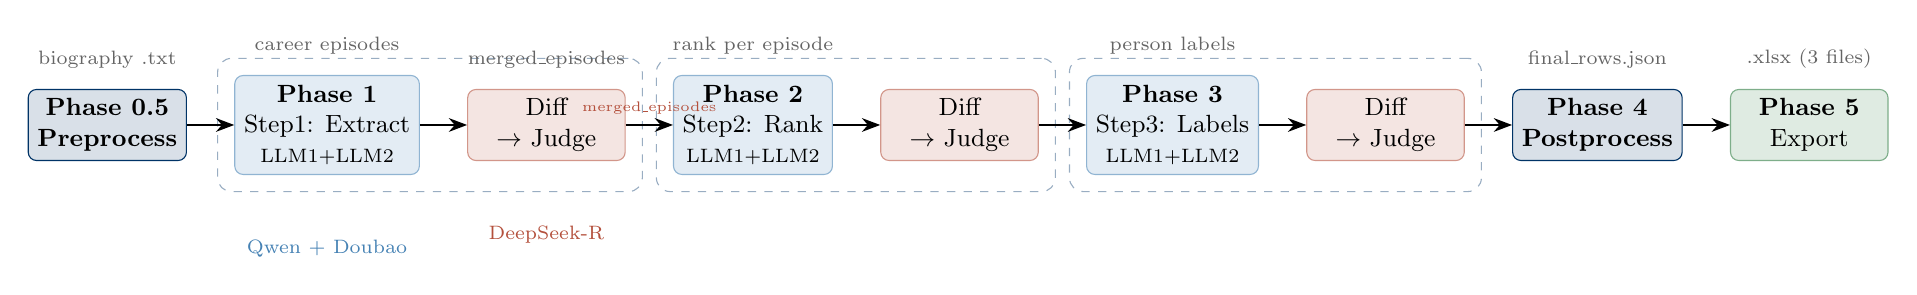
\begin{tikzpicture}[
    node distance=0.4cm and 0.6cm,
    box/.style={draw, rounded corners=3pt, minimum width=2.0cm,
                minimum height=0.7cm, align=center, font=\small,
                fill=stepbg},
    phase/.style={box, fill=darkblue!15, draw=darkblue, font=\small\bfseries},
    parallel/.style={box, fill=llm1color!15, draw=llm1color!60},
    judge/.style={box, fill=judgecolor!15, draw=judgecolor!60},
    output/.style={box, fill=codegreen!15, draw=codegreen!60},
    arr/.style={-Stealth, thick},
    label/.style={font=\scriptsize, text=codegray},
    stepgrp/.style={draw=darkblue!40, dashed, rounded corners=5pt, inner sep=6pt}
  ]
  % Phase 0.5
  \node[phase] (p05) {\textbf{Phase 0.5}\\Preprocess};
  % Phase 1: Step1 extraction
  \node[parallel, right=of p05] (s1llm) {\textbf{Phase 1}\\Step1: Extract\\{\scriptsize LLM1+LLM2}};
  \node[judge, right=of s1llm] (s1j) {Diff\\$\to$ Judge};
  % Phase 2: Step2 rank
  \node[parallel, right=of s1j] (s2llm) {\textbf{Phase 2}\\Step2: Rank\\{\scriptsize LLM1+LLM2}};
  \node[judge, right=of s2llm] (s2j) {Diff\\$\to$ Judge};
  % Phase 3: Step3 labels
  \node[parallel, right=of s2j] (s3llm) {\textbf{Phase 3}\\Step3: Labels\\{\scriptsize LLM1+LLM2}};
  \node[judge, right=of s3llm] (s3j) {Diff\\$\to$ Judge};
  % Phase 4 & 5
  \node[phase, right=of s3j] (p4) {\textbf{Phase 4}\\Postprocess};
  \node[output, right=of p4] (p5) {\textbf{Phase 5}\\Export};
  % Arrows
  \draw[arr] (p05)--(s1llm);
  \draw[arr] (s1llm)--(s1j);
  \draw[arr] (s1j)--(s2llm) node[midway, above, font=\tiny, text=judgecolor]{merged\_episodes};
  \draw[arr] (s2llm)--(s2j);
  \draw[arr] (s2j)--(s3llm);
  \draw[arr] (s3llm)--(s3j);
  \draw[arr] (s3j)--(p4);
  \draw[arr] (p4)--(p5);
  % Group braces for interleaved phases
  \begin{scope}[on background layer]
    \node[stepgrp, fit=(s1llm)(s1j), label={[font=\tiny, text=darkblue]below:Step 1 cycle}] {};
    \node[stepgrp, fit=(s2llm)(s2j), label={[font=\tiny, text=darkblue]below:Step 2 cycle}] {};
    \node[stepgrp, fit=(s3llm)(s3j), label={[font=\tiny, text=darkblue]below:Step 3 cycle}] {};
  \end{scope}
  % I/O labels
  \node[label, above=4pt of p05] {biography .txt};
  \node[label, above=4pt of s1llm] {career episodes};
  \node[label, above=4pt of s1j] {merged\_episodes};
  \node[label, above=4pt of s2llm] {rank per episode};
  \node[label, above=4pt of s3llm] {person labels};
  \node[label, above=4pt of p4] {final\_rows.json};
  \node[label, above=4pt of p5] {.xlsx (3 files)};
  % Models
  \node[label, below=20pt of s1llm, text=llm1color] {Qwen + Doubao};
  \node[label, below=20pt of s1j, text=judgecolor] {DeepSeek-R};
  \end{tikzpicture}}% end resizebox

  \medskip
  \begin{columns}[T]
    \column{0.3\textwidth}
    \textbf{\small Interleaved Design}
    \begin{itemize}\scriptsize
      \item Each step completes its own LLM1+LLM2 $\to$ diff $\to$ judge cycle before the next step begins
      \item Step 2 \& 3 operate on \texttt{merged\_episodes.json} produced by Step 1 judging
    \end{itemize}
    \column{0.35\textwidth}
    \textbf{\small Intermediate Logs} {\scriptsize(per province)}
    \begin{itemize}\tiny
      \item \texttt{logs/\{p\}/preprocessed\_texts.json}
      \item \texttt{logs/\{p\}/llm\{1,2\}\_step1\_results.json}
      \item \texttt{logs/\{p\}/step1\_diff\_report.json}
      \item \texttt{logs/\{p\}/step1\_judge\_decisions.json}
      \item \texttt{logs/\{p\}/merged\_episodes.json}
      \item \texttt{logs/\{p\}/llm\{1,2\}\_step2\_rank.json}
      \item \texttt{logs/\{p\}/step2\_*.json}
      \item \texttt{logs/\{p\}/llm\{1,2\}\_step3\_labels.json}
      \item \texttt{logs/\{p\}/step3\_*.json}
    \end{itemize}
    \column{0.32\textwidth}
    \textbf{\small Final Output} {\scriptsize(per province)}
    \begin{itemize}\tiny
      \item \texttt{output/\{p\}/\{p\}\_officials.xlsx}
      \item \texttt{output/\{p\}/\{p\}\_governors.xlsx}
      \item \texttt{output/\{p\}/\{p\}\_secretaries.xlsx}
      \item \texttt{output/\{p\}/battle.xlsx}
    \end{itemize}
  \end{columns}
\end{frame}

% =============================================================================
\section{Three-Step LLM Extraction}
% =============================================================================

\begin{frame}[shrink=18]{Three-Step Extraction (Phases 1--3, Interleaved)}
  Each step runs LLM1 + LLM2 in parallel $\to$ diff $\to$ judge, \emph{before} the next step begins.
  Steps 2 \& 3 operate on \texttt{merged\_episodes.json} from Step 1 judging.

  \medskip
  \setlength{\columnsep}{10pt}
  \begin{columns}[T,onlytextwidth]
    \column{0.3\textwidth}
    \begin{block}{Step 1 — Career Episodes}
      \small
      Input: numbered lines (L1, L2, \ldots)\\[4pt]
      Output: JSON array of episodes\\[4pt]
      \textbf{Key fields per episode:}
      \begin{itemize}\scriptsize
        \item \texttt{source\_line} (anchor for diff)
        \item Start / end dates (YYYY.MM)
        \item Org tag (33 categories)
        \item Position flag (23 types)
        \item Organization name
        \item Job title
        \item Location (province, city)
        \item Central vs.\ local
      \end{itemize}
    \end{block}

    \column{0.3\textwidth}
    \begin{block}{Step 2 — Administrative Rank}
      \small
      Input: merged episodes\\[4pt]
      Output: rank per episode\\[4pt]
      \textbf{10-level hierarchy:}
      \begin{enumerate}\scriptsize
        \item 正国级 (State level)
        \item 副国级 (Vice-state)
        \item 正部级 (Minister)
        \item 副部级 (Vice-minister)
        \item 正厅级 (Bureau chief)
        \item 副厅级 (Vice-bureau)
        \item 正处级 (Section chief)
        \item 副处级 (Vice-section)
        \item 正科级 / 副科级
        \item 无 (no rank: students, etc.)
      \end{enumerate}
      Special rules for universities, SOEs, courts
    \end{block}

    \column{0.3\textwidth}
    \begin{block}{Step 3 — Person-Level Labels}
      \small
      Input: merged episodes + biography text\\[4pt]
      Output: bio metadata + labels\\[4pt]
      \textbf{Bio fields:}
      \begin{itemize}\scriptsize
        \item Name, birth year, hometown
        \item Ethnic minority (0/1)
        \item Female (0/1)
        \item Full-time bachelor's (0/1)
      \end{itemize}
      \textbf{Analysis labels:}
      \begin{itemize}\scriptsize
        \item Promoted after governor? (1/0/--1/'')
        \item Promoted after party secretary?
        \item Local promotion / local study
        \item Anti-corruption fall? + charges
      \end{itemize}
    \end{block}
  \end{columns}

  \begin{alertblock}{Splitting Rules (Step 1)}
    \scriptsize
    Multiple organizations on one line $\to$ separate episodes \quad|\quad
    Promotion within same org (vice $\to$ full) $\to$ split \quad|\quad
    Admin + party dual post, same org $\to$ may merge \quad|\quad
    Study vs.\ employment $\to$ always separate
  \end{alertblock}
\end{frame}

% =============================================================================
\section{Verification \& Adjudication}
% =============================================================================

\begin{frame}{Verification \& Adjudication (Interleaved per Step)}
  \begin{columns}[T]
    \column{0.48\textwidth}
    \textbf{Per-Step Dual-LLM Cycle}
    \begin{itemize}
      \item For \emph{each} step (1/2/3), \llmone{} and \llmtwo{} run in parallel on the same input
      \item Outputs are diffed field-by-field, keyed on \texttt{source\_line}
      \item Disputes go to \judge{} immediately, \emph{before} the next step begins
      \item Step 2 \& 3 receive \texttt{merged\_episodes.json} (the judged Step 1 output) as input
    \end{itemize}

    \textbf{Judge Adjudication}
    \begin{itemize}
      \item \judge{} = DeepSeek-Reasoner(V3.2)
      \item Receives: extraction rules, both LLM outputs, original biography text
      \item Returns: verdict per disputed field + reasoning
      \item Separate judge decision files per step:\\
            {\scriptsize \texttt{step1\_judge\_decisions.json},
             \texttt{step2\_judge\_decisions.json},
             \texttt{step3\_judge\_decisions.json}}
    \end{itemize}

    \column{0.48\textwidth}
    \begin{block}{Confidence Scoring}
      \begin{tabular}{cl}
        \toprule
        Score & Meaning \\
        \midrule
        100 &  Judge: very confident \\
        90--99 & Judge: strong evidence verdict \\
        75--89 & Judge: moderate confidence \\
        $<75$  & Ambiguous; \\
        \bottomrule
      \end{tabular}
    \end{block}

    \bigskip
    \begin{block}{Battle Table (\texttt{battle.xlsx})}
      \scriptsize
      \begin{tabular}{l}
        Side-by-side: \llmone{} | \llmtwo{} | \judge{} verdict \\
        Judge reasoning per disputed field \\
        Confidence score per episode \\
        Source text excerpt (L编号) \\[2pt]
        \textcolor{alertred}{\textbf{Red rows}} = confidence $< 90\%$ \\
        Exportable for human reviewers
      \end{tabular}
    \end{block}
  \end{columns}
\end{frame}

% =============================================================================
\section{Output Structure}
% =============================================================================

\begin{frame}[shrink=5]{Output: 30-Column Episode Table}
  \begin{columns}[T]
    \column{0.48\textwidth}
    \textbf{Person-level fields} (columns A–N, repeated per episode)
    \begin{center}
    \scriptsize
    \begin{tabular}{lll}
      \toprule
      Col & Field & Example \\
      \midrule
      A & Year (prov.\ tenure start) & 2000 \\
      B & Province & 浙江 \\
      C & Name & 张三 \\
      D & Birth year & 1952 \\
      E & Hometown (province) & 山东 \\
      F & Hometown (city) & 济南 \\
      G & Ethnic minority & 0 \\
      H & Female & 0 \\
      I & Full-time bachelor's & 1 \\
      J & Promoted (governor) & 1 \\
      K & Promoted (party sec.) & -- \\
      L & Local promotion & 0 \\
      M & Local study & 1 \\
      N & Final rank & 副部级 \\
      \bottomrule
    \end{tabular}
    \end{center}

    \column{0.48\textwidth}
    \textbf{Episode-level fields} (columns O–AD, one row per episode)
    \begin{center}
    \scriptsize
    \begin{tabular}{lll}
      \toprule
      Col & Field & Example \\
      \midrule
      O  & Episode \# & 3 \\
      P  & Start date & 1990.03 \\
      Q  & End date & 1995.10 \\
      R  & Org tag & 政府机关 \\
      S  & Position flag & 副职 \\
      T  & Episode rank & 副处级 \\
      U  & Organization & 某省政府 \\
      V  & Job title & 副处长 \\
      W  & Source text excerpt & L4: 任副处长 \\
      X  & Unresolved disputes & -- \\
      Y  & Location (prov.) & 浙江省 \\
      Z  & Location (city) & -- \\
      AA & Central/local & 地方 \\
      AB & Anti-corruption & 否 \\
      AC & Charges detail & -- \\
      AD & Manual review flag & -- \\
      \bottomrule
    \end{tabular}
    \end{center}
  \end{columns}

  \medskip
  \begin{alertblock}{33 Org Categories $\;\cdot\;$ 23 Position Types $\;\cdot\;$ 10 Rank Levels}
    \scriptsize
    Org tags: 党委机关, 政府机关, 人大, 政协, 纪检监察, 法院, 检察院, 军队, 高校, 国有企业, 民主党派, \ldots\\
    Position flags: 正职, 副职, 常委, 委员, 省长/书记 (provincial leader), 学生, 教授, \ldots
  \end{alertblock}
\end{frame}

% =============================================================================
\section{Usage}
% =============================================================================

\begin{frame}[fragile, shrink=5]{Running the Pipeline}
  \begin{columns}[T]
    \column{0.50\textwidth}
    \textbf{Entry point: \texttt{main\_province.py}}

    \begin{lstlisting}[language=bash]
# Single province (uses existing bio files)
uv run main_province.py --province 浙江

# Enable Baidu Baike scraping
uv run main_province.py --province 浙江 --scrape

# Reuse LLM1 results, skip re-extraction
uv run main_province.py --province 浙江 --skip-extract

# Skip judge adjudication
uv run main_province.py --province 浙江 --skip-battle

# Batch: all 31 provinces, 8 parallel workers
uv run main_province.py --batch --workers 8

# Batch: selected provinces
uv run main_province.py --batch \
    --provinces 浙江,北京,广东
    \end{lstlisting}

    \column{0.46\textwidth}
    \begin{block}{Prompt-Driven Configuration}
      \small
      All extraction rules live in \texttt{prompts/}:
      \begin{itemize}\scriptsize
        \item \texttt{step1\_extraction.md}
        \item \texttt{step2\_rank.md}
        \item \texttt{step3\_labeling.md}
        \item \texttt{ref\_university\_rank.md}
        \item \texttt{ref\_soe\_rank.md}
      \end{itemize}
      Modifying behavior = editing \texttt{.md} files only.\\
      Code never hard-codes rule strings.
    \end{block}

    \medskip
    \begin{block}{Model Config (\texttt{config.py})}
      \scriptsize
      \begin{tabular}{ll}
        \textbf{LLM1} & Qwen 3.6-plus (DashScope)\\
        \textbf{LLM2} & Doubao-seed-2.0-pro (Volcengine)\\
        \textbf{Judge} & DeepSeek-Reasoner\\
        \textbf{LLM2 fallback} & Qwen 3.5-plus (DashScope)\\
      \end{tabular}
    \end{block}
  \end{columns}
\end{frame}

% =============================================================================
\section{Quality Assurance}
% =============================================================================

\begin{frame}{Quality Assurance Design}
  \begin{columns}[T]
    \column{0.48\textwidth}
    \textbf{Field-Level Auditability}
    \begin{itemize}
      \item Every extracted field is traceable to a source line (\texttt{source\_line} = L编号)
      \item \texttt{diff\_report.json} records exact LLM1 vs.\ LLM2 values for every disagreement
      \item \texttt{judge\_decisions.json} logs judge verdict \emph{and} reasoning chain
      \item \texttt{[需人工核查]} flag in column AD for edge cases
    \end{itemize}

 

    \column{0.48\textwidth}
    \begin{block}{Key Validation Rules}
      \begin{itemize}\scriptsize
        \item \texttt{source\_line} must be non-null (diff anchor)
        \item Org tags restricted to 33 canonical values
        \item Position flags restricted to 23 canonical values
        \item Location names normalized to official full forms
        \item Ranks from 10-level hierarchy + ``无''
        \item Anti-corruption fields validated against known case records
      \end{itemize}
    \end{block}

    \bigskip
    \begin{block}{Three Sources of Truth}
      \scriptsize
      \begin{tabular}{ll}
        \toprule
        Artifact & Source \\
        \midrule
        Extraction rules & \texttt{prompts/*.md} \\
        Column definitions & \texttt{config.py: COLUMNS} \\
        Official roster & \texttt{data/\{prov\}\_officials.txt} \\
        \bottomrule
      \end{tabular}
    \end{block}
  \end{columns}
\end{frame}

% =============================================================================
\section{Summary}
% =============================================================================

\begin{frame}{Summary}
  \begin{columns}[T]
    \column{0.55\textwidth}
    \textbf{Contributions}
    \begin{enumerate}
      \item \textbf{Scale}: $\sim$600 officials, $\sim$20{,}000 career episodes, 31 provinces
      \item \textbf{Depth}: 30 structured fields per episode, including administrative rank inference (10 levels) and anti-corruption outcomes
      \item \textbf{Reliability}: Two-LLM independent extraction + DeepSeek-Reasoner adjudication with field-level confidence scores
      \item \textbf{Reproducibility}: Prompt-driven rules, read-only raw data, deterministic intermediate JSONs
      \item \textbf{Auditability}: Full reasoning chains, source-line traceability, battle table for manual review
    \end{enumerate}

    \column{0.42\textwidth}
    \begin{block}{Research Applications}
      \begin{itemize}
        \item Career trajectory analysis for Chinese officials
        \item Promotion incentives and local economic performance
        \item Anti-corruption campaign targeting patterns
        \item Factional politics and elite circulation
        \item Local state capacity and institutional change
      \end{itemize}
    \end{block}
  \end{columns}

\end{frame}

% ── Appendix ─────────────────────────────────────────────────────────────────
\appendix

\begin{frame}{Appendix: 33 Organizational Tag Categories}
  \scriptsize
  \begin{columns}[T]
    \column{0.33\textwidth}
    \textbf{Party / State}
    \begin{itemize}
      \item 党委机关 (Party committee)
      \item 政府机关 (Government agency)
      \item 人大 (People's Congress)
      \item 政协 (CPPCC)
      \item 纪检监察 (Discipline inspection)
      \item 组织部 (Organization dept.)
      \item 宣传部 (Propaganda dept.)
      \item 统战部 (United Front)
      \item 政法委 (Political-legal affairs)
    \end{itemize}
    \column{0.33\textwidth}
    \textbf{Judicial / Military}
    \begin{itemize}
      \item 法院 (Court)
      \item 检察院 (Procuratorate)
      \item 军队 (Military)
      \item 武警 (Armed police)
      \item 公安 (Public security)
      \item 司法行政 (Judicial admin.)
    \end{itemize}
    \textbf{Economic}
    \begin{itemize}
      \item 国有企业 (SOE — central)
      \item 地方国企 (SOE — local)
      \item 金融机构 (Financial inst.)
    \end{itemize}
    \column{0.33\textwidth}
    \textbf{Education / Research / Other}
    \begin{itemize}
      \item 高校 (University)
      \item 科研院所 (Research inst.)
      \item 民主党派 (Minor parties)
      \item 群团组织 (Mass organizations)
      \item 媒体 (Media)
      \item 外交机构 (Foreign affairs)
      \item 港澳机构 (HK/Macau affairs)
      \item 援外机构 (Foreign aid)
      \item 其他 (Other)
      \item \ldots
    \end{itemize}
  \end{columns}
\end{frame}

\begin{frame}{Appendix: Administrative Rank Special Rules}
  \begin{block}{Universities}
    \scriptsize
    31 ``A-tier'' universities (985 + key national schools): president/party secretary = 副部级\\
    All other universities accredited by Ministry of Education: president/party secretary = 正厅级\\
    Department chairs: one level below institution rank
  \end{block}

  \smallskip
  \begin{block}{State-Owned Enterprises}
    \scriptsize
    54 central SOEs (国资委 supervised): CEO/board chair = 副部级; vice CEO = 副部级/正厅级\\
    27 central financial enterprises (e.g., Big-4 banks): similar half-level structure\\
    Provincial SOEs: CEO = 正厅级; vice CEO = 副厅级
  \end{block}

  \smallskip
  \begin{block}{Courts \& Procuratorates}
    \scriptsize
    Supreme Court / Supreme Procuratorate: 正部级\\
    Provincial-level court/procuratorate: 正厅级 (half-level above same-level gov. agency)\\
    Municipal/county: same pattern
  \end{block}

  \smallskip
  \begin{block}{Vice-Provincial Cities (副省级城市)}
    \scriptsize
    15 sub-provincial cities (Beijing, Shanghai excluded — already directly administered):\\
    Mayor = 副部级; district/county heads = 正厅级
  \end{block}
\end{frame}

\end{document}
